\documentclass[10pt,conference]{IEEEtran}

% SANER 2027 Agentic AI4SE Track
% Double-anonymous submission
% Main text: maximum 10 pages
% References: up to 2 additional pages

\usepackage{cite}
\usepackage{amsmath,amssymb,amsfonts}
\usepackage{algorithm}
\usepackage{algorithmic}
\usepackage{graphicx}
\usepackage{textcomp}
\usepackage{xcolor}
\usepackage{booktabs}
\usepackage{multirow}
\usepackage{tabularx}
\usepackage{url}
\usepackage[hidelinks]{hyperref}
\usepackage{balance}
\usepackage{placeins}
\usepackage{tikz}

\usetikzlibrary{arrows.meta,positioning,fit,backgrounds,calc}

\newcommand{\blueval}[1]{\textcolor{blue}{#1}}

\def\BibTeX{{\rm B\kern-.05em{\sc i\kern-.025em b}\kern-.08em
T\kern-.1667em\lower.7ex\hbox{E}\kern-.125emX}}

\begin{document}

\title{EvoRationale: A Stateful Agent for Evidence-Grounded
Revalidation of Architectural Decisions during Software Evolution}

% Double-anonymous submission: do not include author names, affiliations,
% acknowledgments, funding details, or identifying links.
\author{\IEEEauthorblockN{Anonymous Authors}}

\maketitle


\begin{abstract}
Architectural decisions often remain in force after the assumptions and evidence that justified them have changed. Existing architecture-recovery, rationale-mining, and traceability techniques recover artifacts or detect structural divergence, but they do not determine whether post-decision evidence continues to support an accepted decision. We formulate \emph{architectural decision revalidation} and \emph{design-rationale drift}, and introduce \textsc{EvoRationale}, a bounded, stateful agent that, given an adjudicated decision state, retrieves temporally eligible artifacts, links them to rationale elements, preserves verified findings across investigation rounds, checks material claims, and recommends \textsc{Keep}, \textsc{Revalidate}, \textsc{Revise}, or \textsc{Reopen} for human review. We evaluate \textsc{EvoRationale} against seven prespecified baselines on 1,200 held-out episodes from 40 repositories across two organizations, using repository-disjoint partitions and shared initial states, model settings, and budgets. \textsc{EvoRationale} achieves drift and outcome macro-F$_1$ scores of 0.82 and 0.79, improving over the prespecified comparator by 0.08 and 0.09. Evidence-retrieval and evidence-link F$_1$ reach 0.84 and 0.78, gains of 0.06 and 0.10, while evaluator-estimated unsupported-claim rate decreases from 0.15 to 0.07. A system-blinded audit corroborates this improvement in grounding: repository-weighted human-adjudicated UCR is 0.086 versus 0.171, a paired absolute reduction of 0.085 (95\% CI [0.062, 0.110]). These gains require 22.8\% more execution time and 21.9\% higher API cost than the stateless tool agent. All five single-component ablations degrade their prespecified target measures, with explicit linking showing the largest conditional contribution. The findings support evidence-grounded post-decision assistance; automatic initial-state construction and practitioner effects remain unevaluated.
\end{abstract}



\begin{IEEEkeywords}
architectural decisions, software evolution, design rationale, agentic AI, evidence grounding, temporal reasoning, software architecture
\end{IEEEkeywords}
 % \vspace{-2mm}

\section{Introduction}
\label{sec:introduction}
Architectural decisions often outlive the conditions that justified them. As systems evolve, workloads, dependencies, requirements, quality priorities, and operational evidence may change even when implementations remain structurally conformant \cite{Lehman1980Programs,Perry1992Foundations,Jansen2005Decisions}. Existing approaches address adjacent concerns: architectural-knowledge and rationale techniques capture or recover decision context \cite{Tang2006Rationale,Demir2024Survey,Santana2026ADR}; architecture recovery and conformance detect implementation divergence \cite{Bucaioni2024Continuous,Su2026Violations}; and traceability and repository-level retrieval locate related artifacts \cite{Fuchss2025Traceability,Akhavan2026LinkAnchor,Wang2026RepoReasoner}. None directly reassesses whether post-acceptance evidence still justifies an accepted decision. We call this task \emph{architectural decision revalidation} and define \emph{design-rationale drift} as a mismatch between recorded rationale and evolved project context.
Revalidation requires more than retrieval. Evidence must fall between decision acceptance and the evaluation cutoff, remain within the repository boundary, identify the evaluated artifact version, and preserve provenance. It must also be linked to the goal, assumption, requirement, constraint, quality attribute, dependency, or prior evidence that it affects. Finally, drift and action must remain distinct: incomplete or conflicting evidence may require further investigation, whereas sufficiently strong evidence may justify revising or reopening a decision. Every material claim must therefore be traceable to eligible evidence.
We present \textsc{EvoRationale}, a bounded, stateful single agent that maintains a versioned decision state, derives unresolved evidence needs, retrieves and links temporally eligible artifacts, classifies their evidential roles, and recommends \textsc{Keep}, \textsc{Revalidate}, \textsc{Revise}, or \textsc{Reopen}. Decision Memory retains verified findings, unresolved questions, rejected interpretations, and verifier feedback across bounded rounds. Deterministic checks validate identifiers, timestamps, provenance, citations, evidence relations, and output structure; Alloy contributes evidence only for formalizable constraints, and humans retain final authority. We evaluate \textsc{EvoRationale} against seven baselines on 1,200 held-out episodes from 40 repository-disjoint projects. Giving every system the same adjudicated $S_0$ isolates revalidation from state construction. \textsc{EvoRationale} improves all six prespecified effectiveness and grounding measures, with the human audit corroborating lower UCR, at higher execution cost. Five full-corpus ablations and an Alloy-subset analysis examine the contributions of components.

\noindent\textbf{Contributions.} This work (1) formulates architectural decision revalidation, six drift categories, and four actionable outcomes; (2) presents a stateful architecture combining decision memory, temporal retrieval, explicit linking, bounded investigation, and verification; (3) constructs a longitudinal, independently annotated benchmark with decision states, ordered evidence, evidence-to-rationale links, evidential relations, drift labels, and outcomes; and (4) provides a repository-disjoint evaluation of effectiveness, grounding, efficiency, cross-organizational variation, and component contributions under controlled inputs and budgets.
\section{Motivating Example and Problem Definition}
\label{sec:motivation-problem}

\subsection{Motivating Example}
\label{sec:motivating-example}

Consider a team that accepts a Redis-based caching decision at time $t_0$ to satisfy a peak-load latency target. Its rationale assumes a predominantly read-heavy workload, infrequent profile updates, and manageable cache invalidation \cite{Bucaioni2024Continuous,Su2026Violations}. After acceptance, stale-data incidents contradict the update assumption, distributed invalidation weakens the expected operational trade-off, and database optimization supersedes the benchmark that originally justified caching (Figure~\ref{fig:motivating-timeline}). At cutoff $t_c$, the implementation may still conform to the selected design, but the combined evidence materially challenges its central justification. No individual artifact determines the outcome: the recommendation to \textsc{Reopen} follows from temporally ordering the evidence and relating each artifact to the specific rationale element it affects.





\begin{figure}[!t]
\centering
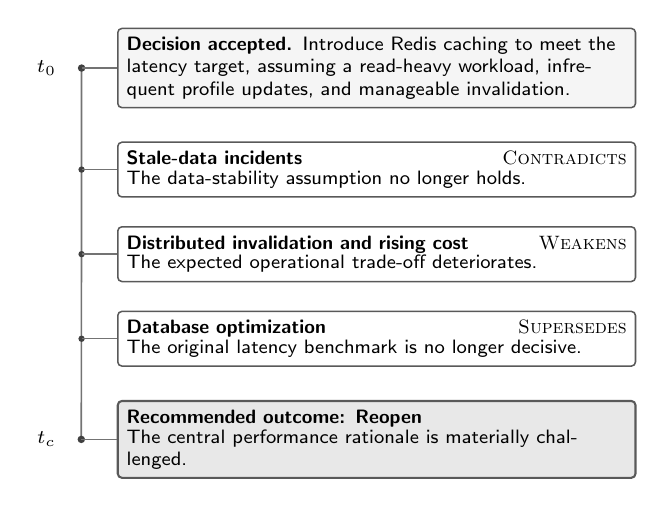
\begin{tikzpicture}[
    font=\sffamily\scriptsize,
    base/.style={
        draw=black!65,
        rounded corners=1.5pt,
        align=left,
        text width=6.35cm,
        minimum width=6.35cm,
        inner sep=3.2pt,
        line width=0.55pt
    },
    decision/.style={base,fill=black!4},
    evidence/.style={base,fill=white},
    outcome/.style={base,fill=black!9,line width=0.75pt},
    time/.style={font=\sffamily\bfseries\scriptsize}
]

\node[decision] (decision) {
    \textbf{Decision accepted.}
    Introduce Redis caching to meet the latency target, assuming a read-heavy workload, infrequent profile updates, and manageable invalidation.
};

\node[evidence, below=4.2mm of decision] (stale) {
    \textbf{Stale-data incidents}
    \hfill \textsc{Contradicts}\\[-0.3mm]
    The data-stability assumption no longer holds.
};

\node[evidence, below=3.6mm of stale] (cost) {
    \textbf{Distributed invalidation and rising cost}
    \hfill \textsc{Weakens}\\[-0.3mm]
    The expected operational trade-off deteriorates.
};

\node[evidence, below=3.6mm of cost] (database) {
    \textbf{Database optimization}
    \hfill \textsc{Supersedes}\\[-0.3mm]
    The original latency benchmark is no longer decisive.
};

\node[outcome, below=4.2mm of database] (outcome) {
    \textbf{Recommended outcome: \textsc{Reopen}}\\[-0.3mm]
    The central performance rationale is materially challenged.
};

\coordinate (m0) at ([xshift=-4.5mm]decision.west);
\coordinate (m1) at ([xshift=-4.5mm]stale.west);
\coordinate (m2) at ([xshift=-4.5mm]cost.west);
\coordinate (m3) at ([xshift=-4.5mm]database.west);
\coordinate (m4) at ([xshift=-4.5mm]outcome.west);

\draw[draw=black!55,line width=0.6pt] (m0) -- (m4);

\fill[black!75] (m0) circle (1.35pt);
\fill[black!75] (m1) circle (1.15pt);
\fill[black!75] (m2) circle (1.15pt);
\fill[black!75] (m3) circle (1.15pt);
\fill[black!75] (m4) circle (1.35pt);

\draw[draw=black!55,line width=0.5pt] (m0) -- (decision.west);
\draw[draw=black!55,line width=0.5pt] (m1) -- (stale.west);
\draw[draw=black!55,line width=0.5pt] (m2) -- (cost.west);
\draw[draw=black!55,line width=0.5pt] (m3) -- (database.west);
\draw[draw=black!55,line width=0.5pt] (m4) -- (outcome.west);

\node[time,anchor=east] at ([xshift=-2mm]m0) {$t_0$};
\node[time,anchor=east] at ([xshift=-2mm]m4) {$t_c$};

\end{tikzpicture}
\caption{Motivating timeline: post-decision evidence weakens or contradicts rationale and leads to \textsc{Reopen} at $t_c$.}

\label{fig:motivating-timeline}
\end{figure}
 % \vspace{-1mm}
\subsection{Architectural Decision Revalidation}
\label{sec:problem-formulation}

Let $d$ denote an architectural decision accepted at time $t_0$. Its initial decision state is
 % \vspace{-2mm}
\begin{equation}
S_0=\langle d,G,\mathcal{R},A,E,Q,C,I\rangle,
\label{eq:decision-state}
\end{equation}

where $G$, $\mathcal{R}$, $A$, $E$, and $Q$ represent the decision's goals, requirements, assumptions, original evidence, and affected quality attributes, respectively. $C$ contains constraints and dependencies, while $I$ records implementation scope and explicit validity conditions. These elements may originate from multiple project artifacts rather than a single architectural decision record \cite{Jansen2005Decisions,Tang2006Rationale,Borowa2023Rationales,Ahmeti2024ADRPractice,Keim2026Scattered}. Let $H_{t_c}=\langle h_1,\ldots,h_n\rangle$ denote the repository history ordered by the earliest verifiable timestamp of each artifact version, with $t_0<\tau(h_i)\leq t_c$. Temporal eligibility is necessary but not sufficient for evidential use: a retained artifact must also be relevant to a state element and assigned an explicit relation from {\emph{supports}, \emph{weakens}, \emph{contradicts}, \emph{supersedes}}. An evidence record preserves the artifact identity, version, timestamp, provenance, affected state element, and assigned relation. Architectural decision revalidation is the mapping
 % \vspace{-1mm}
\begin{equation}
\mathcal{F}(S_0,H_{t_c})\mapsto
O_{t_c}=\langle y,T,E^{*},\mathcal{U},r,a,\mathbf{c}\rangle,
\label{eq:revalidation-output}
\end{equation}

where $y$ is the recommended outcome; $T$ is a multi-label set of detected drift types; $E^{*}$ contains the verified evidence records; $\mathcal{U}$ contains unresolved questions; $r$ is the evidence-grounded rationale; $a$ is the proposed next action; and $\mathbf{c}$ contains the associated confidence scores.  The multi-label set $T$ may contain one or more of six drift types: assumption, evidence, requirement, implementation, quality-attribute, and dependency drift. The recommendation $y$ is one of \textsc{Keep}, \textsc{Revalidate}, \textsc{Revise}, or \textsc{Reopen}; drift type alone does not determine it. \textsc{Keep} indicates that the available evidence continues to support the central rationale and reveals no material reason for change. \textsc{Revalidate} indicates that missing or conflicting evidence prevents a defensible judgment and requires further investigation. \textsc{Revise} indicates that the decision remains defensible, but sufficient evidence requires modification of its scope, conditions, or recorded rationale. \textsc{Reopen} indicates that the central justification is materially weakened, contradicted, or superseded and that alternatives should be reconsidered. Every outcome is a recommendation for human review; $S_0$ becomes a new authoritative state only after human approval.

\section{Related Work}
\label{sec:related-work}

\subsection{Architectural Knowledge, Rationale, and Evolution}

Architectural-decision models organize design context, alternatives, rationale, consequences, and quality trade-offs \cite{Jansen2005Decisions,Tyree2005Decisions,Tang2006Rationale,VanHeesch2012Framework}, while rationale models connect decisions to requirements and design elements \cite{Tang2007Rationale}. In practice, such knowledge is often incomplete, scattered, or lost during software evolution \cite{Tofan2011Vaporization,Demir2024Survey,Ahmeti2024ADRPractice,Santana2026ADR}. Recent LLM-based approaches generate design rationale and architectural decision records (ADRs) or recover architectural documentation and views \cite{Zhou2026Rationale,Gupta2026Context,DeLuca2026CIAO,Miryala2026Views}. Kantara, the closest rationale-mining approach, extracts rationale from commit messages, constructs a knowledge graph, and identifies relationships and potential conflicts among historical decisions \cite{Dhaouadi2025Kantara}. Kantara recovers and relates historical rationale; \textsc{EvoRationale} evaluates whether post-acceptance evidence continues to justify a particular decision. Architecture-recovery and erosion techniques instead detect structural divergence between intended and implemented architectures \cite{DeSilva2012Erosion,Li2022Erosion,Zhang2026SemRef}, including code--documentation inconsistencies and architectural-rule violations \cite{Kiecker2026Cascade,Su2026Violations,Bucaioni2024Continuous}. These techniques assess implementation alignment, whereas revalidation assesses the continuing validity of the decision's evidential basis.

\subsection{Traceability, Retrieval, and Stateful Agents}

Traceability research connects architectural decisions and components to source artifacts \cite{Fuchss2025Traceability}, recovers decisions from communication channels \cite{Soliman2024MailingLists}, and reconstructs issue-to-commit links through repository navigation \cite{Akhavan2026LinkAnchor}. Repository-level reasoning spans files, dependencies, execution behavior, and development history \cite{Jimenez2024SWEBench,Wang2026RepoReasoner}. Tool-using agents support navigation, localization, planning, and modification \cite{Yang2024SWEAgent,Zhang2024AutoCodeRover,Bairi2024CodePlan,Chen2025LocAgent}, while retrieval methods improve context selection through iterative retrieval, component-aware RAG, reranking, adaptive signals, and filtering \cite{Zhang2023RepoCoder,Ke2026RAG,Zhang2025CodeRAG,Shi2026AIRCoder,Huo2026RepoShapley}. These systems generally retrieve or connect artifacts for a current development task. \textsc{EvoRationale} instead derives evidence needs from a historical decision state, restricts retrieval to the decision's post-acceptance interval, and assigns retained artifacts explicit evidential relations to affected rationale elements. Its memory also differs from repair-oriented experience stores such as \textsc{ExpeRepair} \cite{Mu2026ExpeRepair}: rather than transferring repair experiences across tasks, Decision Memory preserves verified evidence, unresolved questions, rejected interpretations, and verifier feedback for one evolving decision.
 % \vspace{-1mm}
\subsection{Verifier-Guided Reasoning}

Verifier-guided agents use external feedback to test and refine generated outputs. Existing approaches incorporate proof-assistant feedback or Alloy counterexamples into iterative correction \cite{Tu2026AgenticVerification,Alhanahnah2025Alloy}. The \textsc{EvoRationale} verifier addresses a different correctness boundary: it validates repository provenance, artifact versions, timestamps, temporal eligibility, citations, evidence relations, and output structure. Alloy is invoked only for formalizable decision constraints, and its instances or counterexamples are treated as evidence rather than architectural verdicts.





\section{The \textsc{EvoRationale} Approach}
\label{sec:approach}

\textsc{EvoRationale} orchestrates retrieval, linking, memory, analysis, and verification as internal tools of one bounded agent. Figure~\ref{fig:evorationale-overview} shows the deployment workflow, and Algorithm~\ref{alg:revalidation-loop} specifies the automatic loop from an available $S_0$, which is also the controlled-evaluation boundary.

\subsection{System Boundary and Orchestration}
\label{sec:architecture-orchestration}

The orchestrator converts unresolved state elements into evidence questions and a structured report. Its outer retrieve--link--verify--update--analyze--validate sequence, checkpoints, and stopping bounds are fixed rather than model-generated. Within this scaffold, the LLM selects and reformulates questions and repository queries, interprets artifacts, classifies evidential relations, and revises its investigation from verifier feedback; it is never treated as evidence. Deterministic gates enforce repository, temporal, and artifact-version boundaries and validate identifiers, provenance, citations, labels, and output structure. The agent cannot alter these boundaries, bypass verification, approve recommendations, or overwrite authoritative state. This bounded agency preserves adaptive investigation while keeping evidential admissibility and architectural authority auditable and outside model control.









\begin{figure*}[!t]
\centering
\resizebox{0.98\textwidth}{!}{%
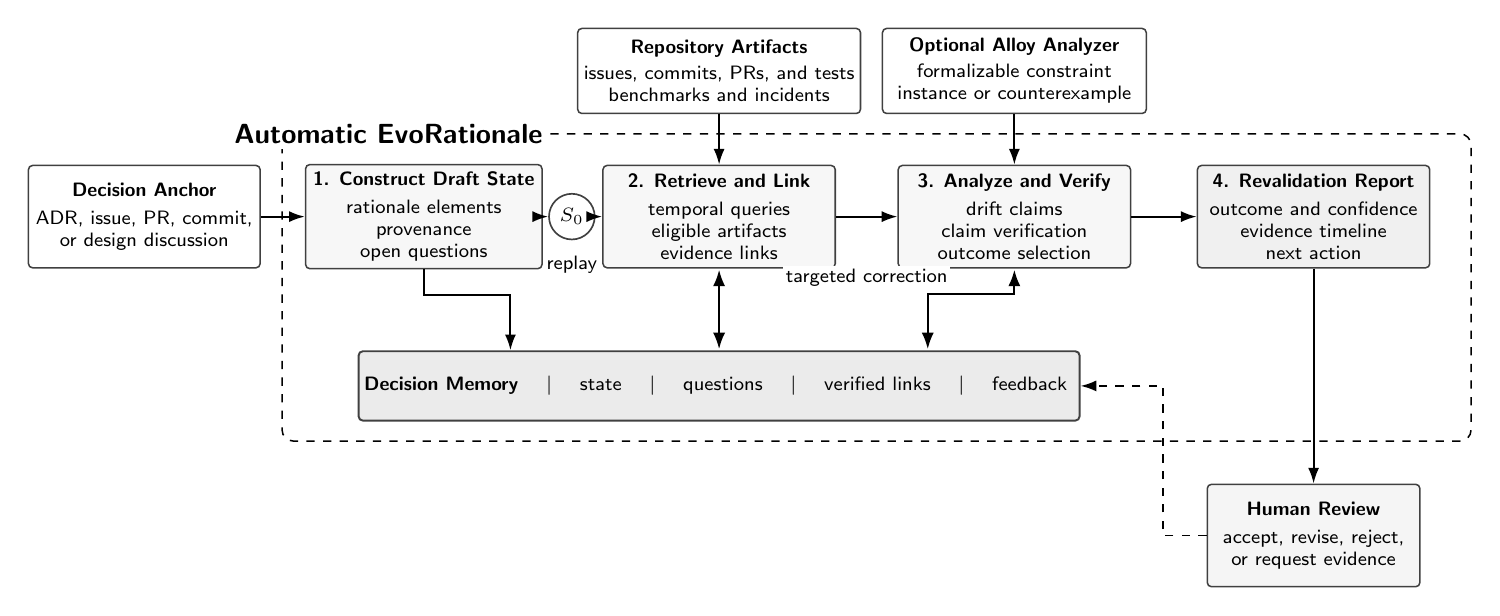
\begin{tikzpicture}[
    x=1cm,
    y=1cm,
    font=\sffamily\scriptsize,
    box/.style={
        draw=black!75,
        rounded corners=1.5pt,
        align=center,
        inner sep=2.7pt,
        minimum height=1.30cm,
        fill=white,
        line width=0.55pt
    },
    stage/.style={
        box,
        minimum width=2.95cm,
        fill=black!3
    },
    ext/.style={
        box,
        minimum width=2.70cm
    },
    support/.style={
        box,
        minimum width=3.35cm,
        minimum height=1.08cm,
        inner sep=2.2pt
    },
    memory/.style={
        box,
        minimum width=8.20cm,
        minimum height=0.88cm,
        inner sep=2pt,
        fill=black!8,
        line width=0.70pt
    },
    gate/.style={
        draw=black!75,
        circle,
        minimum size=0.58cm,
        inner sep=0pt,
        fill=white,
        line width=0.60pt,
        font=\sffamily\scriptsize
    },
    flow/.style={
        -{Latex[length=2mm,width=1.4mm]},
        line width=0.75pt
    },
readwrite/.style={
    <->,
    >={Latex[length=2.1mm,width=1.55mm]},
    line width=0.80pt,
    shorten <=0.4pt,
    shorten >=0.4pt
},
    feedback/.style={
        -{Latex[length=2mm,width=1.4mm]},
        dashed,
        line width=0.70pt
    }
]

\node[ext] (anchor) at (0,0) {
    \textbf{Decision Anchor}\\[0.7mm]
    ADR, issue, PR, commit,\\
    or design discussion
};

\node[stage] (state) at (3.55,0) {
    \textbf{1. Construct Draft State}\\[0.7mm]
    rationale elements\\
    provenance\\
    open questions
};

\node[gate] (s0) at (5.43,0) {$S_0$};

\node[
    font=\sffamily\scriptsize,
    align=center,
    below=0.7mm of s0
] {replay};

\node[stage] (retrieve) at (7.30,0) {
    \textbf{2. Retrieve and Link}\\[0.7mm]
    temporal queries\\
    eligible artifacts\\
    evidence links
};

\node[stage] (analyze) at (11.05,0) {
    \textbf{3. Analyze and Verify}\\[0.7mm]
    drift claims\\
    claim verification\\
    outcome selection
};

\node[stage,fill=black!6] (report) at (14.85,0) {
    \textbf{4. Revalidation Report}\\[0.7mm]
    outcome and confidence\\
    evidence timeline\\
    next action
};

\node[memory] (memory) at (7.30,-2.15) {
    \textbf{Decision Memory}
    \quad $\vert$ \quad state
    \quad $\vert$ \quad questions
    \quad $\vert$ \quad verified links
    \quad $\vert$ \quad feedback
};

\node[support] (repo) at (7.30,1.85) {
    \textbf{Repository Artifacts}\\[0.5mm]
    issues, commits, PRs, and tests\\
    benchmarks and incidents
};

\node[support] (alloy) at (11.05,1.85) {
    \textbf{Optional Alloy Analyzer}\\[0.5mm]
    formalizable constraint\\
    instance or counterexample
};

\node[ext,fill=black!4] (human) at (14.85,-4.05) {
    \textbf{Human Review}\\[0.7mm]
    accept, revise, reject,\\
    or request evidence
};

% Automatic-system boundary
\draw[
    dashed,
    rounded corners=4pt,
    line width=0.55pt
]
    (1.75,1.05) rectangle (16.85,-2.85);

\node[
    fill=white,
    inner sep=1.8pt,
    font=\sffamily\bfseries
]
    at (3.10,1.05)
    {Automatic \textsc{EvoRationale}};

% Main workflow
\draw[flow] (anchor.east) -- (state.west);
\draw[flow] (state.east) -- (s0.west);
\draw[flow] (s0.east) -- (retrieve.west);
\draw[flow] (retrieve.east) -- (analyze.west);
\draw[flow] (analyze.east) -- (report.west);
\draw[flow] (report.south) -- (human.north);

% Decision-memory access
\draw[flow]
    (state.south)
    -- ++(0,-0.32)
    -| ($(memory.north)+(-2.65,0)$);

\draw[readwrite]
    (retrieve.south)
    -- (retrieve.south |- memory.north);

\draw[readwrite]
    (analyze.south)
    -- ++(0,-0.32)
    -| ($(memory.north)+(2.65,0)$);

% External tool inputs enter through their processing stages
\draw[flow]
    (repo.south) -- (retrieve.north);

\draw[flow]
    (alloy.south) -- (analyze.north);

% Verification-driven correction
\draw[feedback]
    (analyze.south west)
    to[out=-145,in=-35,looseness=0.85]
    node[
        midway,
        fill=white,
        inner sep=1pt,
        font=\sffamily\scriptsize
    ] {targeted correction}
    (retrieve.south east);

% Human feedback
\draw[feedback]
    (human.west)
    -- ++(-0.55,0)
    |- (memory.east);

\end{tikzpicture}
}%

\caption{Architecture of \textsc{EvoRationale}. Stage~1 drafts $S_0$, whereas replay uses the shared adjudicated $S_0$. Solid one-way and bidirectional arrows denote workflow and memory access; dashed arrows denote correction or feedback. Only human review updates the authoritative state.}
\label{fig:evorationale-overview}
\end{figure*}

\begin{algorithm}[!t]
\caption{Bounded post-decision revalidation}
\label{alg:revalidation-loop}
\begin{algorithmic}[1]
\REQUIRE Initial state $S_0$, history $H_{t_c}$, interval $(t_0,t_c]$, budget $B$
\ENSURE Evidence-grounded report $R$ for human review

\STATE $M \leftarrow \textsc{InitializeMemory}(S_0)$
\STATE $\mathcal{U} \leftarrow \textsc{FormulateEvidenceNeeds}(S_0)$

\WHILE{$\mathcal{U}\neq\emptyset$ and $\neg\textsc{Stop}(B,M)$}
\STATE $q \leftarrow \textsc{SelectQuestion}(\mathcal{U},M)$
\STATE $X \leftarrow \textsc{Retrieve}(q,H_{t_c},(t_0,t_c],B)$

\STATE $L \leftarrow \textsc{LinkAndClassify}(X,S_0,q)$
\STATE $(L^{+},F_E) \leftarrow \textsc{VerifyEvidence}(L,X)$
\STATE $M \leftarrow \textsc{UpdateMemory}(M,L^{+},F_E)$
\STATE $R \leftarrow \textsc{AnalyzeAndPlan}(S_0,M,\mathcal{U})$
\STATE $(v,F_R) \leftarrow \textsc{ValidateReport}(R,M)$
\STATE $M \leftarrow \textsc{RecordFeedback}(M,F_R)$
\STATE $F \leftarrow F_E \cup F_R$
\STATE $\mathcal{U}\leftarrow
       \textsc{UpdateNeeds}(\mathcal{U},q,L^{+},F)$


\IF{$v=\textsc{Pass}$ and $\mathcal{U}=\emptyset$}
\RETURN $R$
\ENDIF
\ENDWHILE

\RETURN $\textsc{UnresolvedReport}(S_0,M,\mathcal{U})$
\end{algorithmic}
\end{algorithm}
 % \vspace{-2mm}
\subsection{Decision-State Construction and Memory}
\label{sec:decision-state-memory}

During deployment, the Decision-State Builder automatically proposes a draft $S_0$ based on ADRs, issues, pull requests, commits, and design discussions. Each candidate element retains its artifact identifier, version, source location, earliest verifiable timestamp, and extraction confidence. Explicit project statements populate the draft state; unsupported inferences are marked uncertain, and missing rationale becomes an unresolved question rather than fabricated evidence. Human confirmation makes the draft authoritative. The replay evaluation bypasses this construction step and supplies every system with the same adjudicated $S_0$. Decision Memory maintains the resulting working state, evidence needs, verified links, rejected interpretations, verifier feedback, and current assessment without modifying the authoritative state.

\subsection{Temporal Evidence Retrieval and Linking}
\label{sec:temporal-retrieval}

For each unresolved state element, the Temporal Query Planner records the target element, relevant components and artifact types, interval $(t_0,t_c]$, and stopping condition. Repository tools execute these questions iteratively and expand retrieval only when the available evidence or verifier feedback identifies a concrete gap \cite{Akhavan2026LinkAnchor,Zhang2023RepoCoder,Ke2026RAG}. A deterministic temporal gate rejects a candidate unless its exact artifact version belongs to the authorized repository and existed within the eligible interval. The Evidence Linker then records the artifact identifier, version, timestamp, source location, provenance, affected state element, and evidential relation. Only verified links enter Decision Memory. A question is resolved only when sufficient direct evidence passes verification; if repeated searches yield no new relevant artifact or the budget is exhausted, the question remains explicitly unresolved.

\subsection{Drift Analysis, Verification, and Human Review}
\label{sec:drift-verification}

The Drift Analyzer compares $S_0$ with the verified evidence timeline. Every drift claim must identify an affected state element, a supporting artifact, and an explicit evidential relation; a drift category does not directly determine the revalidation outcome. The Action Planner synthesizes verified relations, conflicting evidence, coverage, and unresolved questions to recommend an outcome and next action. The Output Validator checks schemas, labels, identifiers, timestamps, provenance, duplicate references, and confidence ranges. The Evidence Verifier reopens the exact cited artifact versions and checks their content, relevance, timing, and assigned relations. Failed checks become targeted evidence needs for a bounded correction round and cannot be resolved from the LLM's parametric knowledge. For formalizable constraints, Alloy may produce an instance or counterexample \cite{Alhanahnah2025Alloy}; the result is stored with its command, scope, originating state element, and provenance and is treated as evidence rather than an architectural verdict. The final report presents the recommendation, verified evidence, affected elements, unresolved questions, confidence level, and proposed next action for human review.

 % \vspace{-2mm}

\section{Study Design}
\label{sec:study-design}
We evaluate post-decision revalidation through repository-disjoint retrospective replay under shared initial states, immutable snapshots, and budgets. Four RQs examine decision effectiveness, evidence grounding, efficiency, organizational variation, and component contributions.
 % \vspace{-1mm}
\subsection{Research Questions}
\label{sec:research-questions}

\noindent\textbf{RQ1.} How accurately does \textsc{EvoRationale} detect design-rationale drift and predict revalidation outcomes?

\noindent\textbf{RQ2.} How accurately does it retrieve, link, and classify post-decision evidence, and how well does that evidence ground its reports?

\noindent\textbf{RQ3.} What execution overhead does \textsc{EvoRationale} incur relative to the strongest baseline, and how do its outcome performance and report grounding vary between the two organizations?

\noindent\textbf{RQ4.} How much does each architectural component contribute to effectiveness, grounding, and execution efficiency?


\subsection{Benchmark Construction}
\label{sec:benchmark-construction}

We constructed a longitudinal benchmark of 1,500 architectural-decision episodes from 50 proprietary enterprise repositories across two organizations (Table~\ref{tab:benchmark-summary}). Repositories, rather than individual episodes, were the partitioning unit. The organization-stratified development partition contains 300 episodes from 10 repositories, and the held-out partition contains 1,200 episodes from 40 repositories; no repository appears in both. Protocol refinement, prompt selection, and parameter tuning were used only on the development partition. Repository access was restricted to authorized study personnel under applicable data-use agreements. Reporting uses blinded Organization A/B labels and excludes repository, developer, URL, internal identifier, source excerpt, and other identifying information. An episode consists of a decision accepted at $t_0$, an adjudicated initial state $S_0$, an evaluation cutoff $t_c$, and the repository history in $(t_0,t_c]$. The cutoff is the timestamp of the immutable repository snapshot used for replay. It was fixed before evidence and outcome annotation and was not selected according to the presence of drift, the amount or direction of evidence, or the eventual outcome. Consequently, every evaluated configuration receives the same history ending at $t_c$. Decision anchors originate from ADRs, design documents, issues, pull requests, commits, or design discussions. We classify an anchor as explicit when a dedicated project record states the decision and as implicit when linked artifacts jointly establish its acceptance and scope. Both types require at least a partially documented rationale; implementation artifacts alone cannot provide an undocumented justification. Inclusion additionally requires architectural significance, an identifiable acceptance time and implementation scope, and a nonempty eligible post-decision history. Candidate pools were constructed independently of \textsc{EvoRationale} by combining manual repository search with the top 50 BM25 and top 50 BGE-M3 results per query, fused by reciprocal-rank fusion with $k=60$, followed by exact-identifier and repository-link expansion. Search was capped at 12 queries per episode and stopped earlier after all direct links were inspected, and two consecutive reformulations found no new relevant parent artifact. Segments were consolidated by parent-artifact identifier and exact version; overlapping segments counted once, later edits remained distinct, and only versions first auditable in $(t_0,t_c]$ were eligible. Episode selection preceded outcome annotation and did not use revalidation labels. We excluded duplicates, routine refactorings, local implementation choices, and episodes lacking recoverable rationale or adequate history. Each retained episode contains $S_0$, candidate and reference evidence, evidence-to-state links and relations, drift labels, and one reference outcome. Repository-disjoint partitioning prevents project overlap, while the interval $(t_0,t_c]$ prevents pre-decision evidence leakage. During repository screening, we examined 82 repositories (43 from Organization A and 39 from Organization B). We excluded 26 because of incomplete or inaccessible snapshots (7), unverifiable decision-acceptance timestamps (6), fewer than 30 eligible episodes (9), or repository duplication or overlap (4). From the remaining 56 repositories (29/27), an organization-stratified random draw with seed 2027 selected 25 from each organization before annotation. Across these 50 repositories, 3,684 candidate episodes were assigned mutually exclusive reasons for exclusion: duplicates (286), routine refactorings (512), local implementation choices (351), unrecoverable rationale (247), or inadequate post-decision history (141), leaving 2,147 eligible episodes. Forty-four repositories exceeded the prespecified 30-episode cap, and six contained exactly 30. A repository-specific deterministic shuffle, combining seed 2027 with the repository identifier, retained 30 episodes per repository and removed 647, resulting in 1,500 episodes. Within each organization, a seed-2027 draw assigned five repositories to development and the remaining 20 to held-out evaluation before annotation. Organizational balance was imposed by design; outcome frequencies were not sampling quotas.
 % \vspace{-2mm}

\begin{table*}[!t]
\caption{Benchmark composition; parenthesized counts show the A/B split. Outcomes and anchors are exclusive; drift labels are not.}
\label{tab:benchmark-summary}
\centering
\scriptsize
\renewcommand{\arraystretch}{1.04}
\setlength{\tabcolsep}{4pt}
\begin{tabular*}{\textwidth}{@{\extracolsep{\fill}}lclclc@{}}
\toprule
\multicolumn{2}{c}{\textbf{Corpus and Partitions}} &
\multicolumn{2}{c}{\textbf{Held-Out Outcomes and Anchors}} &
\multicolumn{2}{c}{\textbf{Held-Out Drift and Evidence}} \\
\cmidrule(lr){1-2}
\cmidrule(lr){3-4}
\cmidrule(lr){5-6}
\textbf{Characteristic} &
\textbf{Value} &
\textbf{Characteristic} &
\textbf{Episodes / Value} &
\textbf{Characteristic} &
\textbf{Episodes / Value} \\
\midrule
Total repositories
& 50
& \textsc{Keep}
& 338
& Assumption drift
& 420 \\

Organization A / B repositories
& 25 / 25
& \textsc{Revalidate}
& 271
& Evidence drift
& 455 \\

Development repositories
& 10 (5 / 5)
& \textsc{Revise}
& 249
& Requirement drift
& 315 \\

Held-out repositories
& 40 (20 / 20)
& \textsc{Reopen}
& 342
& Implementation drift
& 370 \\

Development episodes
& 300 (150 / 150)
& Explicit-anchor episodes
& 690
& Quality-attribute drift
& 340 \\

Held-out episodes
& 1,200 (600 / 600)
& Implicit-anchor episodes
& 510
& Dependency drift
& 395 \\

Total episodes
& 1,500
& Formalizable episodes / repositories
& 186 / 31
& Median reference evidence per episode
& 8 \\

Pilot episodes
& 60
& Reference-label audit episodes
& 150
& Median post-decision history, months
& 18 \\
\bottomrule
\end{tabular*}
\end{table*}



\subsection{Annotation and Reference Labels}
\label{sec:annotation}

Three software architecture researchers developed the codebook using a stratified pilot of 60 development episodes, with 30 episodes from each organization. The pilot remained in the development partition and was not included in the held-out evaluation. After codebook refinement, the 60 pilot episodes were reannotated under the frozen codebook before tuning. Two researchers independently annotated every non-pilot episode, and the third adjudicated disagreements. Assignments were rotated, and annotators were blinded to system identities and outputs during initial judging. The initial candidate pools, judging rules, and residual-judging protocol were frozen before held-out execution. Artifacts retrieved outside an initial pool were not automatically scored as non-relevant: two source-system-blinded annotators judged them independently, the third adjudicated disagreements, and confirmed relevant artifacts were added to the shared reference set before final scoring of every system. Annotation proceeded in stages: candidate-evidence relevance and affected state element, evidential relation, multi-label drift categories, and finally, one revalidation outcome. Unsupported information was marked uncertain, and missing rationale remained unresolved rather than being inferred from implementation artifacts. Agreement was computed from pre-adjudication labels after the pilot and every 100 episodes using Krippendorff's $\alpha$ \cite{Krippendorff2018ContentAnalysis}. Values of $\alpha\geq0.80$ were accepted; $0.67\leq\alpha<0.80$ triggered targeted review; and $\alpha<0.67$ required codebook revision, additional training, and re-annotation. On the held-out partition, pre-adjudication $\alpha$ was 0.86 for evidence relevance, 0.79 for evidential relations, and 0.83 for outcomes. Binary agreement across the six drift categories ranged from 0.76 to 0.88. Because the evidence links are set-valued, we also report a pairwise F$_1$ score of 0.82 and a Jaccard similarity of 0.71. Relations and drift categories below 0.80 underwent targeted review; no held-out $\alpha$ fell below 0.67. Adjudication retained the original labels, cited evidence, final judgment, and rationale. Finally, the full team audited a stratified sample of 150 episodes---30 development and 120 held-out episodes, or 10\% of the benchmark---selected by organization, anchor type, drift category, and reference outcome. Pilot episodes were excluded from this audit. 
\par\noindent\textit{Grounding-evaluator audit.} Before inspecting system or evaluator outputs, we selected 50 held-out episodes covering all 40 repositories (25 per organization). With seed 2027, SHA-256 ranking chose the lowest-ranked episode per repository and the lexicographically first feasible ten-episode extension satisfying reference-outcome (\textsc{Keep}/\textsc{Revalidate}/\textsc{Revise}/\textsc{Reopen}$=14/11/10/15$), anchor-type (explicit/implicit$=29/21$), and coverage of all six drift categories; categories could co-occur. A second hash selected the same value across 10 repetitions for both systems, yielding 100 reports. Human segmentation removed 11 nonmaterial claims, added 7 missing claims, and split 8 compound claims, increasing the number of extracted claims from 360 to 364. After a 20-claim development calibration, two system-blinded annotators independently assessed claim support against exactly cited artifact versions, and a third adjudicated disagreements. Initial agreement ($\alpha=0.528$) triggered codebook revision, another 20-claim calibration, and full reannotation; final agreement reached $\alpha=0.815$ with 95.9\% exact agreement. The evaluator remained frozen.





\subsection{Baselines and Ablations}
\label{subsec:baselines-ablations}

We compare seven baselines: four controlled configurations, one paper-guided reimplementation, and two task adaptations (Table~\ref{tab:baseline-summary}). All systems receive the same adjudicated $S_0$, repository snapshot, boundary $(t_0,t_c]$, generator model, inference settings, output schema, context limit, and episode budget; tool-using systems also share query and unique-artifact-read limits. They differ in evidence retrieval, organization, linking, analysis, and verification. No adaptation receives \textsc{EvoRationale}'s Decision Memory or verifier. \par\noindent\textit{Kantara-Reimplemented.} Because the released materials lack a pinned end-to-end workflow, we follow the paper and available artifacts \cite{Dhaouadi2025Kantara}. The reimplementation processes all temporally eligible, nonempty human-authored commit-message sentences after deterministic boilerplate and duplicate removal, without relevance or label filtering. It retains decision/rationale extraction, the Rationale and Decision Graph, \texttt{has\_rationale}, \emph{Similar}/\emph{Contradicts} relations, and structure-based conflict detection. Adaptations add only the shared boundaries, the $S_0$ mapping, the provenance/version fields, and the report schema. Published examples were reproduced structurally, but not with exact probabilities or aggregate results; two researchers inspected 20 development episodes, followed by a third researcher's review. \par\noindent\textit{LinkAnchor-Adapted.} We validated the executable components of the official \texttt{fse26} implementation before adapting them through a private evaluation fork \cite{Akhavan2026LinkAnchor}, retaining dynamic commit-chain search, lazy tools, aggregate resolution reasoning, \texttt{Store}/\texttt{Discard} feedback, context pruning, Git/diff and issue functions, and Tree-sitter navigation. An adapter maps $S_0$ to the issue interface and restricts retrieval to $(t_0,t_c]$; eligible unique commits in the explored chain form the evidence set, and changed components/files plus shared identifiers or rationale determine artifact--element links. Only the interface, model, and budgets are replaced.

\par\noindent\textit{ExpeRepair-Adapted.} A private fork of upstream \texttt{main} replaces the Test and Patch Agents with Evidence Investigation and Revalidation Reasoning while retaining dynamic prompt composition \cite{Mu2026ExpeRepair}. Frozen episodic and semantic memories are generated without substantive manual editing from system trajectories for all 300 development episodes, including the 60 pilot episodes; BM25 retrieves the top three episodic demonstrations. The memories contain no adjudicated evidence, reference outcomes, gold drift labels, gold evidence links, or held-out information. Links are produced only through the shared output prompt, without an adapter or separate linker. \par\noindent\textit{Selection protocol.} Each system receives 24 candidates evaluated on the same 60 pilot episodes reannotated under the frozen codebook, yielding $1{,}440$ configuration--episode cases per system without held-out use. Selection maximizes the prespecified unweighted mean of drift macro-F$_1$, outcome macro-F$_1$, evidence F$_1$, evidence-link F$_1$, relation macro-F$_1$, and $1-\mathrm{UCR}$. Ties favor a lower UCR, a higher evidence-link F$_1$, lower cost, lower time, and a smaller configuration ID. Each case permits an initial attempt and two transient-failure retries; unrecovered cases receive zero on all five F$_1$ measures and UCR$=1$, and candidates with more than 5\% failures are ineligible. Configurations and primary comparators are frozen before held-out execution: the stateless tool agent for drift, outcome, relation, and UCR, and LinkAnchor-Adapted for evidence and linking, preventing post-hoc selection.



\begin{table*}[!t]
\caption{Baseline configurations. Links denote a method-specific explicit linker beyond the shared output prompt; Partial denotes relational representation, and Reimpl. denotes a paper-guided reimplementation.}
\label{tab:baseline-summary}
\centering
\small
\setlength{\tabcolsep}{4pt}
\begin{tabularx}{\textwidth}{@{}>{\raggedright\arraybackslash}p{2.90cm}>{\raggedright\arraybackslash}p{1.55cm}>{\raggedright\arraybackslash}X>{\raggedright\arraybackslash}p{1.75cm}cc@{}}
\toprule
\textbf{System} & \textbf{Type} & \textbf{Post-decision evidence strategy} & \shortstack[l]{\textbf{State/}\\\textbf{Memory}} & \textbf{Links} & \textbf{Verifier} \\
\midrule
Decision-only LLM & Controlled & Receives no post-decision repository evidence. & None & No & No \\
Long-context LLM & Controlled & Receives eligible artifacts that fit within one context window. & None & No & No \\
Hybrid-RAG & Controlled & Combines lexical and dense retrieval through reciprocal-rank fusion and one-shot generation \cite{Wang2026RepoReasoner,Ke2026RAG}. & None & No & No \\
Kantara-Reimplemented & Reimpl. & Extracts rationale and relations from commit messages using a paper-guided reimplementation \cite{Dhaouadi2025Kantara}. & Rationale graph & Partial & No \\
LinkAnchor-Adapted & Adapted & Retains lazy, dynamic commit-chain search and maps eligible explored-chain commits to explicit decision-element links \cite{Akhavan2026LinkAnchor}. & Execution-local & Yes & No \\
ExpeRepair-Adapted & Adapted & Retrieves from frozen episodic and semantic memories constructed on development episodes \cite{Mu2026ExpeRepair}. & Dual memory & No & No \\
Stateless tool agent & Controlled & Uses the shared repository tools and may reformulate queries within one execution. & None & No & No \\
\textsc{EvoRationale} & Proposed & Uses temporal retrieval, iterative investigation, explicit linking, and verifier-guided correction. & Decision-centered & Yes & Yes \\
\bottomrule
\end{tabularx}
\end{table*}
For RQ4, five one-component ablations remove Decision Memory, iterative retrieval, runtime verification, the lower temporal bound $t_0$, or explicit evidence linking. All retain the complete system's $S_0$, model settings, snapshot, cutoff $t_c$, schema, context limit, and budget, and receive no reference evidence or labels. \emph{Without Temporal Filter} may admit versions available at or before $t_0$ but preserves $t_c$, testing historical inadmissibility rather than post-cutoff or label leakage. Their primary metrics are outcome macro-F$_1$, evidence F$_1$, UCR, drift macro-F$_1$, and evidence-link F$_1$, respectively. The Alloy analysis, also fixed before held-out inspection, compares outcome macro-F$_1$ and UCR on formalizable episodes.



\subsection{Implementation and Experimental Setup}\label{subsec:implementation}
\noindent\textit{Evaluation boundary and representation.} Replay operated on immutable repository snapshots under the shared inputs and budgets defined above. The deployment path normalizes authenticated GitHub and Jira webhooks into versioned Kafka events, but live ingestion, event relevance, automatic decision matching, network delay, and concurrency were outside the evaluation \cite{GitHubWebhookValidation2026,GitHubWebhookHandling2026,AtlassianJiraWebhooks2026,Kreps2011Kafka,ApacheKafkaDesign2026}. MongoDB stored versioned states, evidence, verifier feedback, and run metadata, while Elasticsearch indexed artifacts and extracted architecture facts. Except for the \emph{Without Temporal Filter} ablation, an artifact version was eligible only if its first auditable availability timestamp lay in $(t_0,t_c]$. We used the introducing commit for commits and file versions; the creation or edit timestamp for issue, pull-request, review, and comment versions; and the first timestamp at which a test, benchmark, or incident record was stored in an authorized source. Embedded execution or occurrence times were retained as event metadata but could not backdate eligibility. Later edits formed new versions. The Java and Spring Boot prototype uses Spoon for program structure and framework components and dedicated parsers for manifests, configurations, deployment descriptors, API specifications, and database migrations \cite{Pawlak2016Spoon}. Artifacts were segmented at semantic boundaries; units over 1,024 tokens were divided into segments of at most 1,024 tokens with a 128-token overlap, while retaining parent identifiers and provenance for artifact-level consolidation.\par
\noindent\textit{Retrieval and model configuration.} Artifact embeddings used pinned BAAI/bge-m3 model and tokenizer revisions, 1,024-dimensional normalized vectors, and an 8,192-token encoder limit \cite{Chen2024BgeM3}. Each query retrieved at most 50 BM25 and 50 dense candidates, fused by reciprocal-rank fusion with $k=60$ \cite{Cormack2009RRF,ElasticHybridSearch2026}. A development-selected frozen reranking policy used component overlap, repository links, artifact type, and consistency with the target decision element. The long-context baseline performed no query-based retrieval: eligible segments were ordered in reverse chronological order, ties were resolved by artifact type and stable identifier, and whole segments were packed deterministically within the shared input budget; segments exceeding the remaining budget were omitted rather than truncated. All LLM-based configurations used \texttt{gpt-5.6-terra} through the OpenAI Responses API with \texttt{reasoning.effort=medium}, \texttt{text.verbosity=low}, \texttt{max\_output\_tokens=4096}, and a cumulative 64,000-token input budget per episode \cite{OpenAIModels2026,OpenAIModelGuidance2026}. Each episode allowed one initial round and at most two correction rounds, for at most three retrieve--link--verify rounds, twelve repository queries, and twenty-four unique artifact reads. Execution stopped after verified evidence sufficiency, repeated searches with no new relevant artifact, or budget exhaustion; unresolved needs remained explicit.\par
\noindent\textit{Verification and Alloy.} Before a memory update, the Evidence Verifier reopened each linked artifact version and checked repository scope, temporal eligibility, provenance, content relevance, affected state element, and evidential relation; only passing links entered Decision Memory. After analysis, the Output Validator checked the report schema, labels, identifiers, citations, confidence values, and support for material claims. Failed checks produced explicit feedback and consumed the remaining correction budget. For formalizable constraints, Alloy Analyzer 6.2.0 recorded the originating state element, constraint, command, scope, result, counterexample, and provenance \cite{Jackson2012SoftwareAbstractions,AlloyTools2026}. Alloy output was treated as evidence rather than a revalidation verdict, and human review and authoritative state updates remained outside replay.\par
\noindent\textit{Controls and reproducibility.} All parameters were selected on development repositories and frozen before held-out execution. Ten runs per episode--configuration pair logged prompts, retrieval settings, tool interactions, cited artifact versions, tokens, latency, retries, verifier results, and cost; requests excluded complete proprietary files, credentials, internal URLs, and unrelated content. A planned anonymous artifact will include code, prompts, configurations, the codebook, 24 structurally faithful synthetic episodes with inputs, evidence, links, relations, and labels, pseudonymized repository-level scores, de-identified run-level outputs, and analysis scripts; confidentiality precludes replay on real evidence. Experiments ran sequentially on Ubuntu 24.04 on a 32-core server with 256 GB of memory and an RTX 6000 Ada GPU.\par




\subsection{Evaluation Metrics}
\label{subsec:evaluation-metrics}
\noindent\textit{Runs and aggregation.} We evaluate 1,200 held-out episodes at the decision, artifact, link, and report-claim levels. The complete system and five full-corpus ablations produced $6\times1{,}200\times10=72{,}000$ runs, and the seven baselines produced $7\times1{,}200\times10=84{,}000$ runs. Disabling Alloy added $186\times10=1{,}860$ runs; the corresponding complete-system runs were reused, yielding 157,860 held-out evaluation runs; development tuning cases and retry attempts are excluded from this count. Metrics intended to characterize one execution are computed separately for each repetition. For each repository, we compute the metric over its episodes within each repetition, then average the 10 repetition-specific scores; the reported score is the unweighted mean of the 40 repository scores. Thus, repetitions quantify stochastic variation rather than form a ten-run ensemble. The Alloy analysis applies the same procedure to 186 episodes from 31 repositories. Modal outcomes are used only for recommendation-change counts: an ablation counts as changed when its modal label differs from the complete system's modal label, and the rate is divided by 1,200. A frequency tie is resolved in favor of the tied label with the highest mean confidence among repetitions predicting that label; no tie occurred.
\par\noindent\textit{Drift and outcome prediction (RQ1).} Drift detection is a six-label task evaluated primarily by macro-F$_1$, with micro-F$_1$, Jaccard similarity, exact-set accuracy, and per-category F$_1$ as secondary measures \cite{Sokolova2009Measures}. Outcome prediction is a four-class task evaluated primarily by macro-F$_1$, with balanced accuracy, accuracy, and per-class F$_1$ as secondary measures. Macro-F$_1$ averages the fixed label sets defined in Section~\ref{sec:problem-formulation}, and zero denominators are assigned zero. For \textsc{EvoRationale} and the prespecified stateless-tool comparator, outcome calibration uses each run's four-class probability vector to compute the multiclass Brier score $\sum_{c=1}^{4}(p_c-y_c)^2$ and top-label expected calibration error (ECE) with 15 fixed equal-width bins \cite{Guo2017Calibration}. Unrecovered runs remain in both measures with the uniform vector $(0.25,0.25,0.25,0.25)$. Both measures are descriptive and pool run--episode predictions using inverse-repository-size weights so that repositories contribute equally.
\par\noindent\textit{Evidence retrieval and linking (RQ2).} For run $r$ of episode $j$, let $E_j^{\mathrm{ref}}$ be the final nonempty shared artifact set after adjudication and residual judging, $\widehat{E}_{jr}$ the retained artifact set, and $x_{jr}=|\widehat{E}_{jr}\cap E_j^{\mathrm{ref}}|$. Artifact-level scores are
\begin{equation}
\resizebox{0.90\columnwidth}{!}{$\displaystyle P_{E,jr}=\frac{x_{jr}}{|\widehat{E}_{jr}|},\quad R_{E,jr}=\frac{x_{jr}}{|E_j^{\mathrm{ref}}|},\quad F_{1,E,jr}=\frac{2P_{E,jr}R_{E,jr}}{P_{E,jr}+R_{E,jr}}$}
\label{eq:evidence-metrics}
\end{equation}
All three scores are set to zero when $\widehat{E}_{jr}=\varnothing$; $F_1$ is also zero when $P+R=0$. Because scores follow the aggregation order above, aggregate F$_1$ is not recomputed from aggregate precision and recall. We also report Precision@$10$, Recall@$10$, and nDCG@$10$ with binary relevance after consolidating segments from the same parent artifact \cite{Jarvelin2002NDCG}. Link scoring requires an exact artifact--decision-element pair, whereas relation scoring requires an exact artifact--element--relation triple; an incorrect element or relation contributes one false positive and the corresponding false negative. The relation macro-F$_1$ averages the four fixed relation classes. Before verifier correction, temporal validity is the proportion of proposed links whose exact artifact version belongs to the target repository and first became auditable in $(t_0,t_c]$; provenance completeness is the proportion containing the required identifier, type, location, revision, and timestamp. Citation accuracy is the proportion of report citations whose content, provenance, and interpretation are verified, and evidence coverage is the proportion of adjudicated outcome-relevant artifacts validly cited.
\par\noindent\textit{Grounding.} Material claims comprise evidence relations, drift claims, and factual assertions. An offline evaluator, isolated from runtime verifier outputs, marks a claim as supported only when it is grounded by an eligible cited artifact whose verified content and relation entail the claim, a reproducible Alloy result, or retained provenance that directly restates $S_0$; $S_0$ cannot support post-decision or drift claims. For every report $q$,
\begin{equation}
\mathrm{UCR}_{q}=\frac{N_{\mathrm{unsupported},q}}{N_{\mathrm{material},q}},
\label{eq:ucr}
\end{equation}
where lower values indicate stronger grounding. The output schema requires at least one material claim; a zero-claim or invalid report is assigned UCR$=1$ and counted separately as a report failure. UCR is computed per run and follows the aggregation order above rather than pooling claims. The system-blinded grounding audit above provides human validation of the frozen evaluator; full-corpus UCR remains evaluator-estimated. Outcome correctness is evaluated separately under RQ1.
\par\noindent\textit{Efficiency and ablations (RQ3--RQ4).} Efficiency is measured by model invocations, wall-clock time, and estimated API cost for one episode-level run. The ten values for each episode--configuration pair are averaged; reported time and cost therefore describe one execution, not the sum of repetitions. Ablations are reported as absolute changes from the complete system in their prespecified primary measures and as descriptive changes in the remaining measures. Alloy is analyzed only on formalizable episodes.
\par\noindent\textit{Statistical analysis.} The repository is the unit of inference. We compute 95\% percentile intervals from 10,000 repository-level bootstrap resamples using seed 2027. Full-corpus resamples draw 40 repositories with replacement and retain all of their episodes; Alloy resamples the 31 eligible repositories. Paired intervals use identical sampled repository indices and the empirical 2.5th and 97.5th percentiles of the paired differences. Two-sided Wilcoxon signed-rank tests compare 40 paired repository scores, or 31 for Alloy. The grounding audit applies the same paired bootstrap to its 40 unrounded repository-score pairs; it adds no hypothesis test. Pratt's method retains zero differences during ranking but excludes them from the signed-rank sums, and ties receive average ranks \cite{Pratt1959ZerosTies}. We report $r_{\mathrm{rb}}=(W^{+}-W^{-})/(W^{+}+W^{-})$ \cite{Kerby2014SimpleDifference}, orienting positive values toward \textsc{EvoRationale} in baseline comparisons and the complete system in ablations; lower-is-better measures are reversed. Holm correction controls the familywise error rate at 0.05 within the prespecified RQ1 (two tests), RQ2 (four tests), and RQ4 (seven tests) families; RQ3 adds no tests. Although the Alloy analysis was fixed before held-out inspection, no separate correction family was specified; its two tests therefore join the five full-corpus ablation tests in the RQ4 family \cite{Holm1979Procedure}. We interpret adjusted $p$-values together with confidence intervals, effect sizes, and absolute differences.





\section{Results}
\label{sec:results}
Unless stated otherwise, metrics, confidence intervals, and tests follow the repository-level procedure in Section~\ref{subsec:evaluation-metrics}.
\subsection{RQ1: Drift Detection and Revalidation Outcomes}
\label{subsec:results-rq1}
Table~\ref{tab:rq1-primary} reports the primary RQ1 results. \textsc{EvoRationale} obtains drift macro-F$_1=0.82$ and outcome macro-F$_1=0.79$. Relative to the prespecified stateless-tool comparator, the paired absolute improvements are 0.08 for drift (95\% CI [0.06, 0.10]; $p_{\mathrm{Holm}}=0.004$; $r_{\mathrm{rb}}=0.54$) and 0.09 for outcome prediction ([0.07, 0.11]; $p_{\mathrm{Holm}}=0.002$; $r_{\mathrm{rb}}=0.59$). Secondary drift metrics are micro-F$_1=0.84$, Jaccard similarity $=0.76$, and exact-set accuracy $=0.64$; outcome accuracy and balanced accuracy are 0.81 and 0.79. For outcome calibration, Brier score/ECE are 0.24/0.06 for \textsc{EvoRationale} versus 0.36/0.11 for the stateless comparator; no hypothesis test was performed.
\begin{table}[!t]
\caption{Repository-weighted held-out RQ1 results; bold and underlined values denote the best and second-best, respectively.}
\label{tab:rq1-primary}
\centering
\footnotesize
\renewcommand{\arraystretch}{1.05}
\setlength{\tabcolsep}{4pt}
\begin{tabular}{@{}lcc@{}}
\toprule
\textbf{System}&\textbf{Drift macro-F$_1$}&\textbf{Outcome macro-F$_1$}\\
\midrule
Decision-only LLM&0.42&0.39\\
Long-context LLM&0.58&0.55\\
Hybrid-RAG&0.66&0.63\\
Kantara-Reimplemented&0.56&0.52\\
LinkAnchor-Adapted&0.69&0.64\\
ExpeRepair-Adapted&0.72&0.68\\
Stateless tool agent&\underline{0.74}&\underline{0.70}\\
\textbf{\textsc{EvoRationale}}&\textbf{0.82}&\textbf{0.79}\\
\bottomrule
\end{tabular}
\end{table}
Table~\ref{tab:rq1-breakdown} reports label-level performance. Assumption and evidence drift achieve the highest F$_1$ scores, whereas requirement and quality-attribute drift are less accurately detected. Among outcomes, \textsc{Keep} and \textsc{Reopen} perform best. The confusion matrix shows that \textsc{Revalidate} and \textsc{Revise} are most frequently confused when the evidence establishes an outdated or incomplete rationale but does not clearly distinguish between further investigation and an immediate modification.
\begin{table}[!t]
\caption{Label-level RQ1 performance of \textsc{EvoRationale}.}
\label{tab:rq1-breakdown}
\centering
\scriptsize
\renewcommand{\arraystretch}{1.05}
\setlength{\tabcolsep}{3.2pt}
\begin{tabular}{@{}lclc@{}}
\toprule
\textbf{Drift type}&\textbf{F$_1$}&\textbf{Outcome}&\textbf{F$_1$}\\
\midrule
Assumption&0.85&\textsc{Keep}&0.83\\
Evidence&0.84&\textsc{Revalidate}&0.74\\
Requirement&0.78&\textsc{Revise}&0.72\\
Implementation&0.81&\textsc{Reopen}&0.86\\
Quality attribute&0.79&&\\
Dependency&0.83&&\\
\midrule
\textbf{Macro average}&\textbf{0.82}&\textbf{Macro average}&\textbf{0.79}\\
\bottomrule
\end{tabular}
\end{table}
% \noindent\textbf{Answer to RQ1.} \textsc{EvoRationale} significantly improves both drift detection and outcome prediction over the prespecified comparator; distinguishing \textsc{Revalidate} from \textsc{Revise} remains its principal outcome-classification challenge.
\subsection{RQ2: Evidence Retrieval, Linking, and Grounding}
\label{subsec:results-rq2}
Table~\ref{tab:rq2-results} reports the primary RQ2 measures. For evidence retrieval and linking, the prespecified comparator is LinkAnchor-Adapted. \textsc{EvoRationale} improves evidence F$_1$ from 0.78 to 0.84 (paired $\Delta=0.06$; 95\% CI [0.04, 0.08]; $p_{\mathrm{Holm}}=0.009$; $r_{\mathrm{rb}}=0.46$) and evidence-link F$_1$ from 0.68 to 0.78 ($\Delta=0.10$; [0.08, 0.12]; $p_{\mathrm{Holm}}=0.003$; $r_{\mathrm{rb}}=0.57$). For relation classification and grounding, the prespecified comparator is the stateless tool agent. Relation macro-F$_1$ increases from 0.67 to 0.76 ($\Delta=0.09$; [0.07, 0.11]; $p_{\mathrm{Holm}}=0.006$; $r_{\mathrm{rb}}=0.55$), while evaluator-estimated UCR decreases from 0.15 to 0.07, an absolute reduction of 0.08 and a relative reduction of 53.3\% (95\% CI for the paired reduction [0.06, 0.10]; $p_{\mathrm{Holm}}=0.001$; $r_{\mathrm{rb}}=0.62$).
\begin{table*}[!t]
\caption{Repository-weighted held-out RQ2 results. Aggregate F$_1$ is not recomputed from aggregate precision and recall; UCR is evaluator-estimated, and lower is better. Bold and underlined values denote the best and second-best results, respectively.}
\label{tab:rq2-results}
\centering
\scriptsize
\renewcommand{\arraystretch}{1.06}
\setlength{\tabcolsep}{3.8pt}
\begin{tabular*}{\textwidth}{@{\extracolsep{\fill}}lcccccccccc@{}}
\toprule
\multirow{2}{*}{\textbf{System}}&\multicolumn{3}{c}{\textbf{Evidence Retrieval}}&\multicolumn{3}{c}{\textbf{Evidence Linking}}&\multicolumn{3}{c}{\textbf{Relation Classification}}&\multirow{2}{*}{\textbf{UCR}}\\
\cmidrule(lr){2-4}\cmidrule(lr){5-7}\cmidrule(lr){8-10}
&\textbf{P}&\textbf{R}&\textbf{F$_1$}&\textbf{P}&\textbf{R}&\textbf{F$_1$}&\textbf{P}&\textbf{R}&\textbf{F$_1$}&\\
\midrule
Decision-only LLM&0.00&0.00&0.00&0.00&0.00&0.00&0.00&0.00&0.00&0.61\\
Long-context LLM&0.46&0.66&0.54&0.37&0.43&0.40&0.41&0.45&0.43&0.31\\
Hybrid-RAG&0.74&0.70&0.72&0.57&0.53&0.55&0.61&0.57&0.59&0.22\\
Kantara-Reimplemented&0.51&0.37&0.43&0.44&0.35&0.39&0.52&0.45&0.48&0.34\\
LinkAnchor-Adapted&0.75&\underline{0.81}&\underline{0.78}&0.65&\underline{0.72}&\underline{0.68}&0.66&0.62&0.64&0.19\\
ExpeRepair-Adapted&0.76&0.70&0.73&0.66&0.60&0.63&0.68&0.64&0.66&0.17\\
Stateless tool agent&\underline{0.78}&0.74&0.76&\underline{0.67}&0.63&0.65&\underline{0.69}&\underline{0.65}&\underline{0.67}&\underline{0.15}\\
\textbf{\textsc{EvoRationale}}&\textbf{0.86}&\textbf{0.82}&\textbf{0.84}&\textbf{0.81}&\textbf{0.75}&\textbf{0.78}&\textbf{0.78}&\textbf{0.74}&\textbf{0.76}&\textbf{0.07}\\
\bottomrule
\end{tabular*}
\end{table*}
At rank cutoff 10, \textsc{EvoRationale} obtains Precision@$10=0.83$, Recall@$10=0.88$, and nDCG@$10=0.86$, versus 0.76, 0.81, and 0.79 for LinkAnchor-Adapted. Temporal validity, provenance completeness, citation accuracy, and evidence coverage are 0.97, 0.99, 0.95, and 0.96. The system-blinded audit corroborates UCR: repository-weighted evaluator estimates are 0.075 and 0.158, and human-adjudicated values are 0.086 and 0.171, for \textsc{EvoRationale} and the stateless agent, respectively. The paired human reduction is 0.085 (95\% repository-bootstrap CI [0.062, 0.110]), or 49.9\%. Across 364 claims, evaluator balanced accuracy is 0.892, \textsc{Unsupported}-class F$_1$ is 0.837, and evaluator--human $\kappa=0.815$. Errors primarily involve unrelated component mentions, derivative artifacts, and indirect changes in quality priority.


\subsection{RQ3: Execution Overhead and Cross-Organizational Variation}
\label{subsec:results-rq3} 
Table~\ref{tab:rq3-efficiency} reports the mean held-out resources per episode-level run. Wall-clock time spans the first agent operation through the validated report, including held-out retrieval, model and verifier calls, corrections, retries, and local processing. Cost applies the August 7, 2026, prices to recorded held-out tokens \cite{OpenAIModels2026}. Both measures exclude one-time ingestion, indexing, and embedding generation; all configuration-selection executions and retries on development data; the one-time construction of ExpeRepair-Adapted's frozen episodic and semantic memories from 300 development episodes; and hardware, storage, and human review. Accordingly, RQ3 compares steady-state held-out execution rather than total lifecycle cost.
\begin{table}[!b]
\caption{Mean held-out resources per episode-level run; lower is better.}
\label{tab:rq3-efficiency}
\centering
\scriptsize
\renewcommand{\arraystretch}{1.03}
\setlength{\tabcolsep}{3pt}
\begin{tabularx}{\columnwidth}{@{}Xrrr@{}}
\toprule
\textbf{System}&\textbf{Calls}&\textbf{Time (s)}&\textbf{Cost (\$)}\\
\midrule
Decision-only LLM&1.0&12.4&0.021\\
Long-context LLM&1.0&41.2&0.082\\
Hybrid-RAG&1.0&48.7&0.094\\
Kantara-Reimplemented&1.4&36.1&0.061\\
LinkAnchor-Adapted&2.9&62.4&0.118\\
ExpeRepair-Adapted&2.6&75.8&0.139\\
Stateless tool agent&3.1&84.6&0.151\\
\textsc{EvoRationale}&3.6&103.9&0.184\\
\bottomrule
\end{tabularx}
\end{table}
At \$0.184 and 103.9 seconds per run, the projected monthly cost and sequential time for revalidating $D$ decisions $m$ times are $C_{\mathrm{month}}=0.184Dm$ USD and $T_{\mathrm{seq}}=103.9Dm$ seconds; for $D=100$ and $m=1$, these equal \$18.40 and 2.89 sequential hours. This projection excludes lifecycle costs and does not measure deployment throughput. \par Outcome macro-F$_1$ is 0.80 (95\% CI [0.77, 0.83]) in Organization A and 0.77 ([0.74, 0.80]) in Organization B; evaluator-estimated UCR is 0.06 ([0.04, 0.08]) and 0.08 ([0.06, 0.10]), respectively. The absolute gaps are 0.03 and 0.02. These descriptive estimates show no large observed divergence but do not establish equivalence.
% \par\noindent\textbf{Answer to RQ3.} \textsc{EvoRationale} improves effectiveness and grounding at a higher held-out per-run resource cost. The modest observed organizational gaps remain descriptive rather than evidence of equivalence.

\subsection{RQ4: Component Contributions}
\label{subsec:results-rq4}
Table~\ref{tab:rq4-ablation} summarizes the five full-corpus effects. Every repository-bootstrap interval excludes zero, and all five effects remain significant under the seven-test RQ4 Holm correction ($p_H\leq0.018$); explicit linking produces the largest change.

\begin{table}[!b]
\caption{Full-corpus ablations ($\Delta=$ ablation minus complete); UCR is evaluator-estimated, $p_H$ is Holm-adjusted over all seven RQ4 tests, and $r_{\mathrm{rb}}>0$ favors complete.}
\label{tab:rq4-ablation}
\centering
\scriptsize
\renewcommand{\arraystretch}{1.03}
\setlength{\tabcolsep}{1.5pt}
\begin{tabularx}{\columnwidth}{@{}>{\raggedright\arraybackslash}Xlccc@{}}
\toprule
\textbf{Removed}&\textbf{Target}&\textbf{$\Delta$ [95\% CI]}&\textbf{$p_H$}&\textbf{$r_{\mathrm{rb}}$}\\
\midrule
Decision Memory&Outcome F$_1$&$-0.07$ [$-0.09,-0.05$]&0.018&0.48\\
Iterative retrieval&Evidence F$_1$&$-0.08$ [$-0.10,-0.06$]&0.007&0.52\\
Runtime verification&UCR&$+0.09$ [$+0.07,+0.11$]&0.002&0.61\\
Temporal filtering&Drift F$_1$&$-0.06$ [$-0.08,-0.04$]&0.010&0.50\\
Explicit linking&Link F$_1$&$-0.14$ [$-0.17,-0.11$]&$<0.001$&0.68\\
\bottomrule
\end{tabularx}
\end{table}
On 186 formalizable episodes from 31 repositories, disabling Alloy reduces outcome macro-F$_1$ from 0.81 to 0.78 ($\Delta=-0.03$, 95\% CI [$-0.05,-0.01$]; raw $p=0.018$; $p_{\mathrm{Holm}}=0.036$; $r_{\mathrm{rb}}=0.36$), remaining significant under the seven-test RQ4 correction. Its evaluator-estimated UCR increase from 0.06 to 0.07 is not significant ($\Delta=+0.01$, [$-0.003,+0.023$]; raw $p=0.110$; $p_{\mathrm{Holm}}=0.110$; $r_{\mathrm{rb}}=0.22$). Subset effects are not directly comparable with full-corpus ablations.

\section{Discussion}
\label{sec:discussion}
\noindent\textit{Interpretation.} The contribution is not a new retrieval, memory, or verification primitive, but their decision-centered composition under explicit temporal and evidential constraints. The ablation pattern suggests complementary roles: memory preserves unresolved context across rounds, whereas explicit links and runtime verification constrain which artifacts may justify each claim. The recurring confusion between \textsc{Revalidate} and \textsc{Revise} further shows that successful retrieval does not eliminate architectural judgment when evidence is incomplete or supports modification without invalidating a decision's central rationale.\par\noindent\textit{Operational use.} The measured overhead favors event-triggered use after incidents, dependency or security changes, regressions, or requirement revisions rather than continuous reanalysis. Reports should therefore expose cited evidence, provenance, uncertainty, and unresolved questions, while architects retain authority over stakeholder and organizational trade-offs. Decision records that preserve assumptions, constraints, evidence, alternatives, and validity conditions provide stronger inputs for such revalidation \cite{Jansen2005Decisions,Tyree2005Decisions}.\par\noindent\textit{Contribution boundary.} The controlled replay establishes comparative task accuracy, grounding, and per-run cost; it does not establish practitioner usefulness, architectural decision quality, or time savings.


\section{Threats to Validity}
\label{sec:threats}
\noindent\textit{Construct validity.} Evidence relevance, drift, outcomes, claim segmentation, and support remain interpretive despite frozen codebooks, independent annotation, adjudication, and agreement assessment \cite{Krippendorff2018ContentAnalysis}. The 50-episode audit shows strong but imperfect evaluator--human agreement; full-corpus and ablation UCR depend on generalization beyond audited reports. Reference pools may omit artifacts, and adjudicated $S_0$ excludes state construction and practitioner utility.\par\noindent\textit{Internal validity.} Timestamp error, leakage, hindsight, undocumented context, and model variation may affect replay. Repository-disjoint partitions, immutable snapshots, fixed cutoffs and configurations, and the exclusion of reference labels from system inputs mitigate, but cannot eliminate, these risks. \par\noindent\textit{Comparison validity.} No prior system directly implements revalidation; Kantara is reimplemented, while LinkAnchor and ExpeRepair are adapted. Section~\ref{subsec:baselines-ablations} records the mechanisms retained and replaced. Shared inputs, model settings, budgets, tuning, and frozen held-out configurations reduce implementation bias. Source-paper scores are not compared across different tasks, datasets, and models. The stateless tool agent is the comparator for drift, outcome, relation, and UCR; LinkAnchor-Adapted is the comparator for evidence and linking. Results apply only to these configurations and do not establish inferiority on native tasks. Missing Kantara components, domain shift, and unretained revisions limit fidelity and reconstruction. \par\noindent\textit{Statistical conclusion validity.} Repository-level inference and Holm adjustment address clustering and multiplicity, but 40 repositories, or 31 for Alloy, limit power. Secondary measures are descriptive. Combinatorial removals were not evaluated; single-component ablations estimate conditional removal effects and neither identify component interactions nor justify additive attribution. \par\noindent\textit{External validity.} Two proprietary organizations and a Java/Spring prototype limit generalization. Balanced sampling and the 30-episode cap preclude prevalence estimates; broader and live settings require evaluation. \par\noindent\textit{Reliability and reproducibility.} Confidentiality prevents release of real episodes, evidence, and claim-level audit records, precluding independent evidence-level replay. Synthetic cases and de-identified outputs support pipeline and statistical reproduction but not benchmark representativeness; hosted-model updates and unretained baseline revisions preclude identical reruns.



\vspace{-2mm}
\section{Conclusion}
\label{sec:conclusion}
Architectural decisions can remain structurally implemented even after the evidence supporting them has changed. This work formulates architectural decision revalidation and presents \textsc{EvoRationale}, a bounded, stateful agent that connects temporally admissible repository evidence to the rationale elements it affects. In repository-disjoint replay, \textsc{EvoRationale} improved all six prespecified effectiveness and grounding measures, while the human audit corroborated its lower unsupported-claim rate. The ablations indicate that decision memory, iterative retrieval, temporal filtering, explicit linking, and runtime verification each contribute conditionally within the evaluated configuration; the measured overhead favors selective rather than continuous use. These findings support evidence-grounded decision assistance, not autonomous architectural governance. Future work should evaluate automatic initial-state construction, practitioner outcomes, broader technology settings, live operation, and full-lifecycle cost.\par\noindent\textit{Data availability.} An anonymous replication artifact is under preparation; real study data remain confidential.



\bibliographystyle{IEEEtran}
\balance
\bibliography{references}
\end{document}



